\section{Introduction à l'étude}
\subsection{Sujet de l'étude}
L'objet de cette étude est d'évaluer différentes technologies permettant de mettre en place des connexions sécurisées via des Réseaux Privés Virtuels (VPN). L'objectif est de recenser plusieurs solutions fonctionnant sur divers systèmes d'exploitation et de les confronter entre-elles. Les différentes solutions seront d'abord évaluées en termes de complexité d'installation et d'administration, puis en termes de performances et de facilité d'utilisation.

VPN, ou Réseau Privé Virtuel, est le nom donné à une technologie permettant de relier des machines de façon sécurisée à travers un réseau non sûr comme Internet. Ce travail est effectué en vue de mettre en place une telle solution d'accès au sein de l'ISIMA. Les avantages d'une telle installation seraient multiples, du fait de la possibilité d'accéder au réseau interne de l'école depuis l'extérieur dans les mêmes conditions que si l'on était à l'intérieur.

Deux catégories de solutions VPN existent. On distingue les plate-formes dédiées tels les concentrateurs que les grands équipementiers proposent, et les solutions logicielles disponibles sur les systèmes d'exploitation courants : Microsoft a sa solution, le monde de l'Open-Source également.

Trois architecture ont donc été étudiées afin d'être en accord avec la diversité des solutions existantes : un routeur CISCO 2811XM configuré pour faire du VPN, un WindowsServer2K3 avec les services requis pour établir de connexions VPN, ainsi qu'un serveur Linux CentOS 5.1 avec le logiciel libre OpenVPN. La mise en place d'une plate-forme de test sera au coeur de cette étude.

% \subsection{Contexte de travail}
\subsection{Architecture étudiée}
\subsubsection{Schéma logique}

Le travail a été intégralement réalisé dans la salle A214 de l'école. Nous avons pu mettre en place une maquette complète, permettant de simuler les accès depuis Internet vers un réseau interne. La figure \ref{schema-logique-maquette} présente un schéma logique de la maquette.

\begin{figure}[H]
	\begin{center}
% 		\includegraphics[width=\textwidth]{partie_1/images/schema_logique_maquette.JPG}\\
	\end{center}
	\caption{Schéma logique de la maquette}
	\label{schema-logique-maquette}
\end{figure}

\subsubsection{Schéma physique}

Pour faire cohabiter physiquement les trois architectures ensembles nous avons dû faire des conscessions. La plus importante a consisté à récupérer en DHCP les adresses IP des interfaces connectées au réseau de l'ISIMA, dans un coucis d'interropérabilité. La figure \ref{schema-physique-maquette} illustre l'architecture mise en place :

\begin{figure}[H]
	\begin{center}
	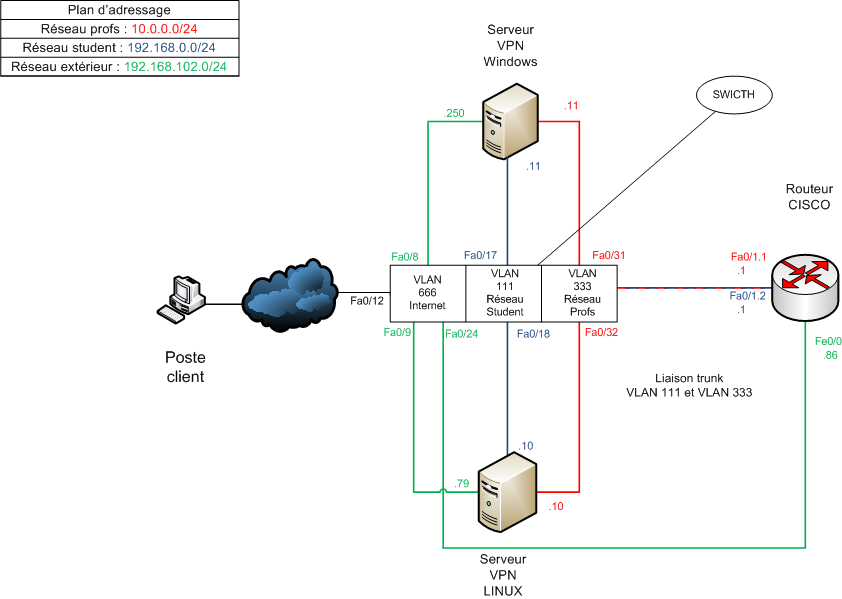
\includegraphics[width=\textwidth]{partie_1/images/archi_phy.png}\\
	\end{center}
	\caption{Schéma physique de la maquette}
	\label{schema-physique-maquette}
\end{figure}

\subsection{Etat de l'art}

\subsubsection{Les différents types de VPN}

Comme expliqué précédemment, un VPN est une technologie permettant de créer des connexions sécurisés à travers un réseau non sûr. Pour cela il existe deux types de mises en place, chacune ayant sa finalité : les VPN bridgés et les VPN routés. Les VPN bridgés sont généralement utilisés lors de connexions site-à-site, tandis que les VPN routés sont eux préférés pour connecter des clients nomades. La mise en place d'un VPN routé s'impose donc pour cette étude, car en plus d'être facilement intégrable à l'architecture existante, elle est parfaitement adaptée à l'usage que l'ISIMA pourrait en faire.

\subsubsection{Les classes de protocoles}
\paragraph{IPsec}
~

IPsec est une suite protocolaire de niveau 3, visant à apporter la sécurité manquant au protocole IP. Cette suite utilise plusieurs protocoles au cours des différentes phases de mise en place d'IPsec.

La première phase est une phase négociation au cours de laquelle les parties se mettent d'accord sur les algorithmes de chiffrement à utiliser et échangent des clefs de session via le protocole ISAKMP (Internet Security Association and Key Management Protocol). Au cours de cette phase le protocole IKE (Internet Key Exchange) intervient également pour générer ces clefs de session soit grâce à une clef partagée soit à l'aide de certificats RSA.

La seconde phase est la phase de communication au cours de laquelle les données peuvent traverser le tunnel et sont chiffrées. Deux protocoles peuvent intervenir en fonction de la finalité du tunnel : ESP qui fournit à la fois intégrité et confidentialité des données, et AH qui fournit l'intégrité et l'authentification.

\paragraph{PPTP}
~

\paragraph{TLS}
~

\subsection{Objectifs fixés}
Recenser les technologies de VPN, mettre en place une maquette de test, confronter les différentes solutions.

\pagebreak
